\begin{flushright} {\tiny {\color{gray} benchmark\_jump2D.tex}} \end{flushright}
%~~~~~~~~~~~~~~~~~~~~~~~~~~~~~~~~~~~~~~~~~~~~~~~~~~~~~~~~~~~~~~~~~~~~~~~~~~~~~~~~~~~~~~~~~~~~~~~~~~

This benchmark is featured in \textcite{sedu23} (2023) 
but orginates in \textcite{wakh13} (2013).
The domain is $\Omega=[0,2]\times[-0.5,1.5]$ and the viscosity is 
given by $\eta(x,y)=\eta_1$ if $y\le 0.5$
and $\eta(x,y)=\eta_2$ if $y > 0.5$.
The analytical solution is given by
\begin{equation}
\vec\upnu=(1-\exp(\lambda)\sin(2\pi y) , 0) 
\qquad
p=\frac12 \exp(2\lambda x)
\qquad
\text{with}
\qquad
\lambda = \frac{1}{2\eta}-\sqrt{\frac{1}{4\eta^2}+4\pi^2}
\end{equation}
The pressure and the gradient tensor exhibit a discontinuity across the interface
Dirichlet boundary conditions are imposed in the whole boundary.

\begin{center}
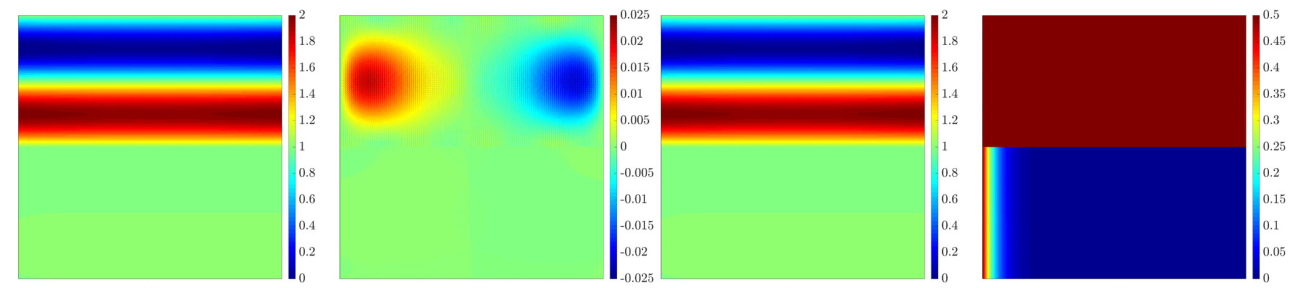
\includegraphics[width=15cm]{images/mms/sedu23a}\\
{\captionfont Taken from \cite{sedu23}. From left to right: 
$u$, $v$, $|\vec\upnu|$, $p$, for $\eta_1=1$ and $\eta=10^{-4}.$}
\end{center}


